\chapter{Our results}

In this chapter we are going to present our results. First some remarks about resolution and convergence of the shape within Auriga simulations for DM and MHD. Then we study the radial and historic profiles of DM and MHD halos, where we obtain the expected tendence found by Vera-Ciro et al. 2011. Then present our principal results, which are the ones referring the comparison DM-MHD.

\section{Analysis of convergence}
We decided to analyze de radial profiles at redshift 0 and compare level5 to level3 simulations. In general, the DM halo shapes remain unchanged with the exeption of the radial regimes where resolution becomes important. However, for MHD simulations, the resolution of gas affects the measurement not only in the inner parts, where resolution issues are evident, but it has a more global effect, presumably because of the scattering of particles which is also supporting the claim that matter affects the halo shape through scattering.\\

We address this problem by performing random sampling of the level3 simulations to reproduce level4 measurements and estimate the associated error.\\

\begin{figure}[!ht]
  \centering
  \subfloat[MHD]{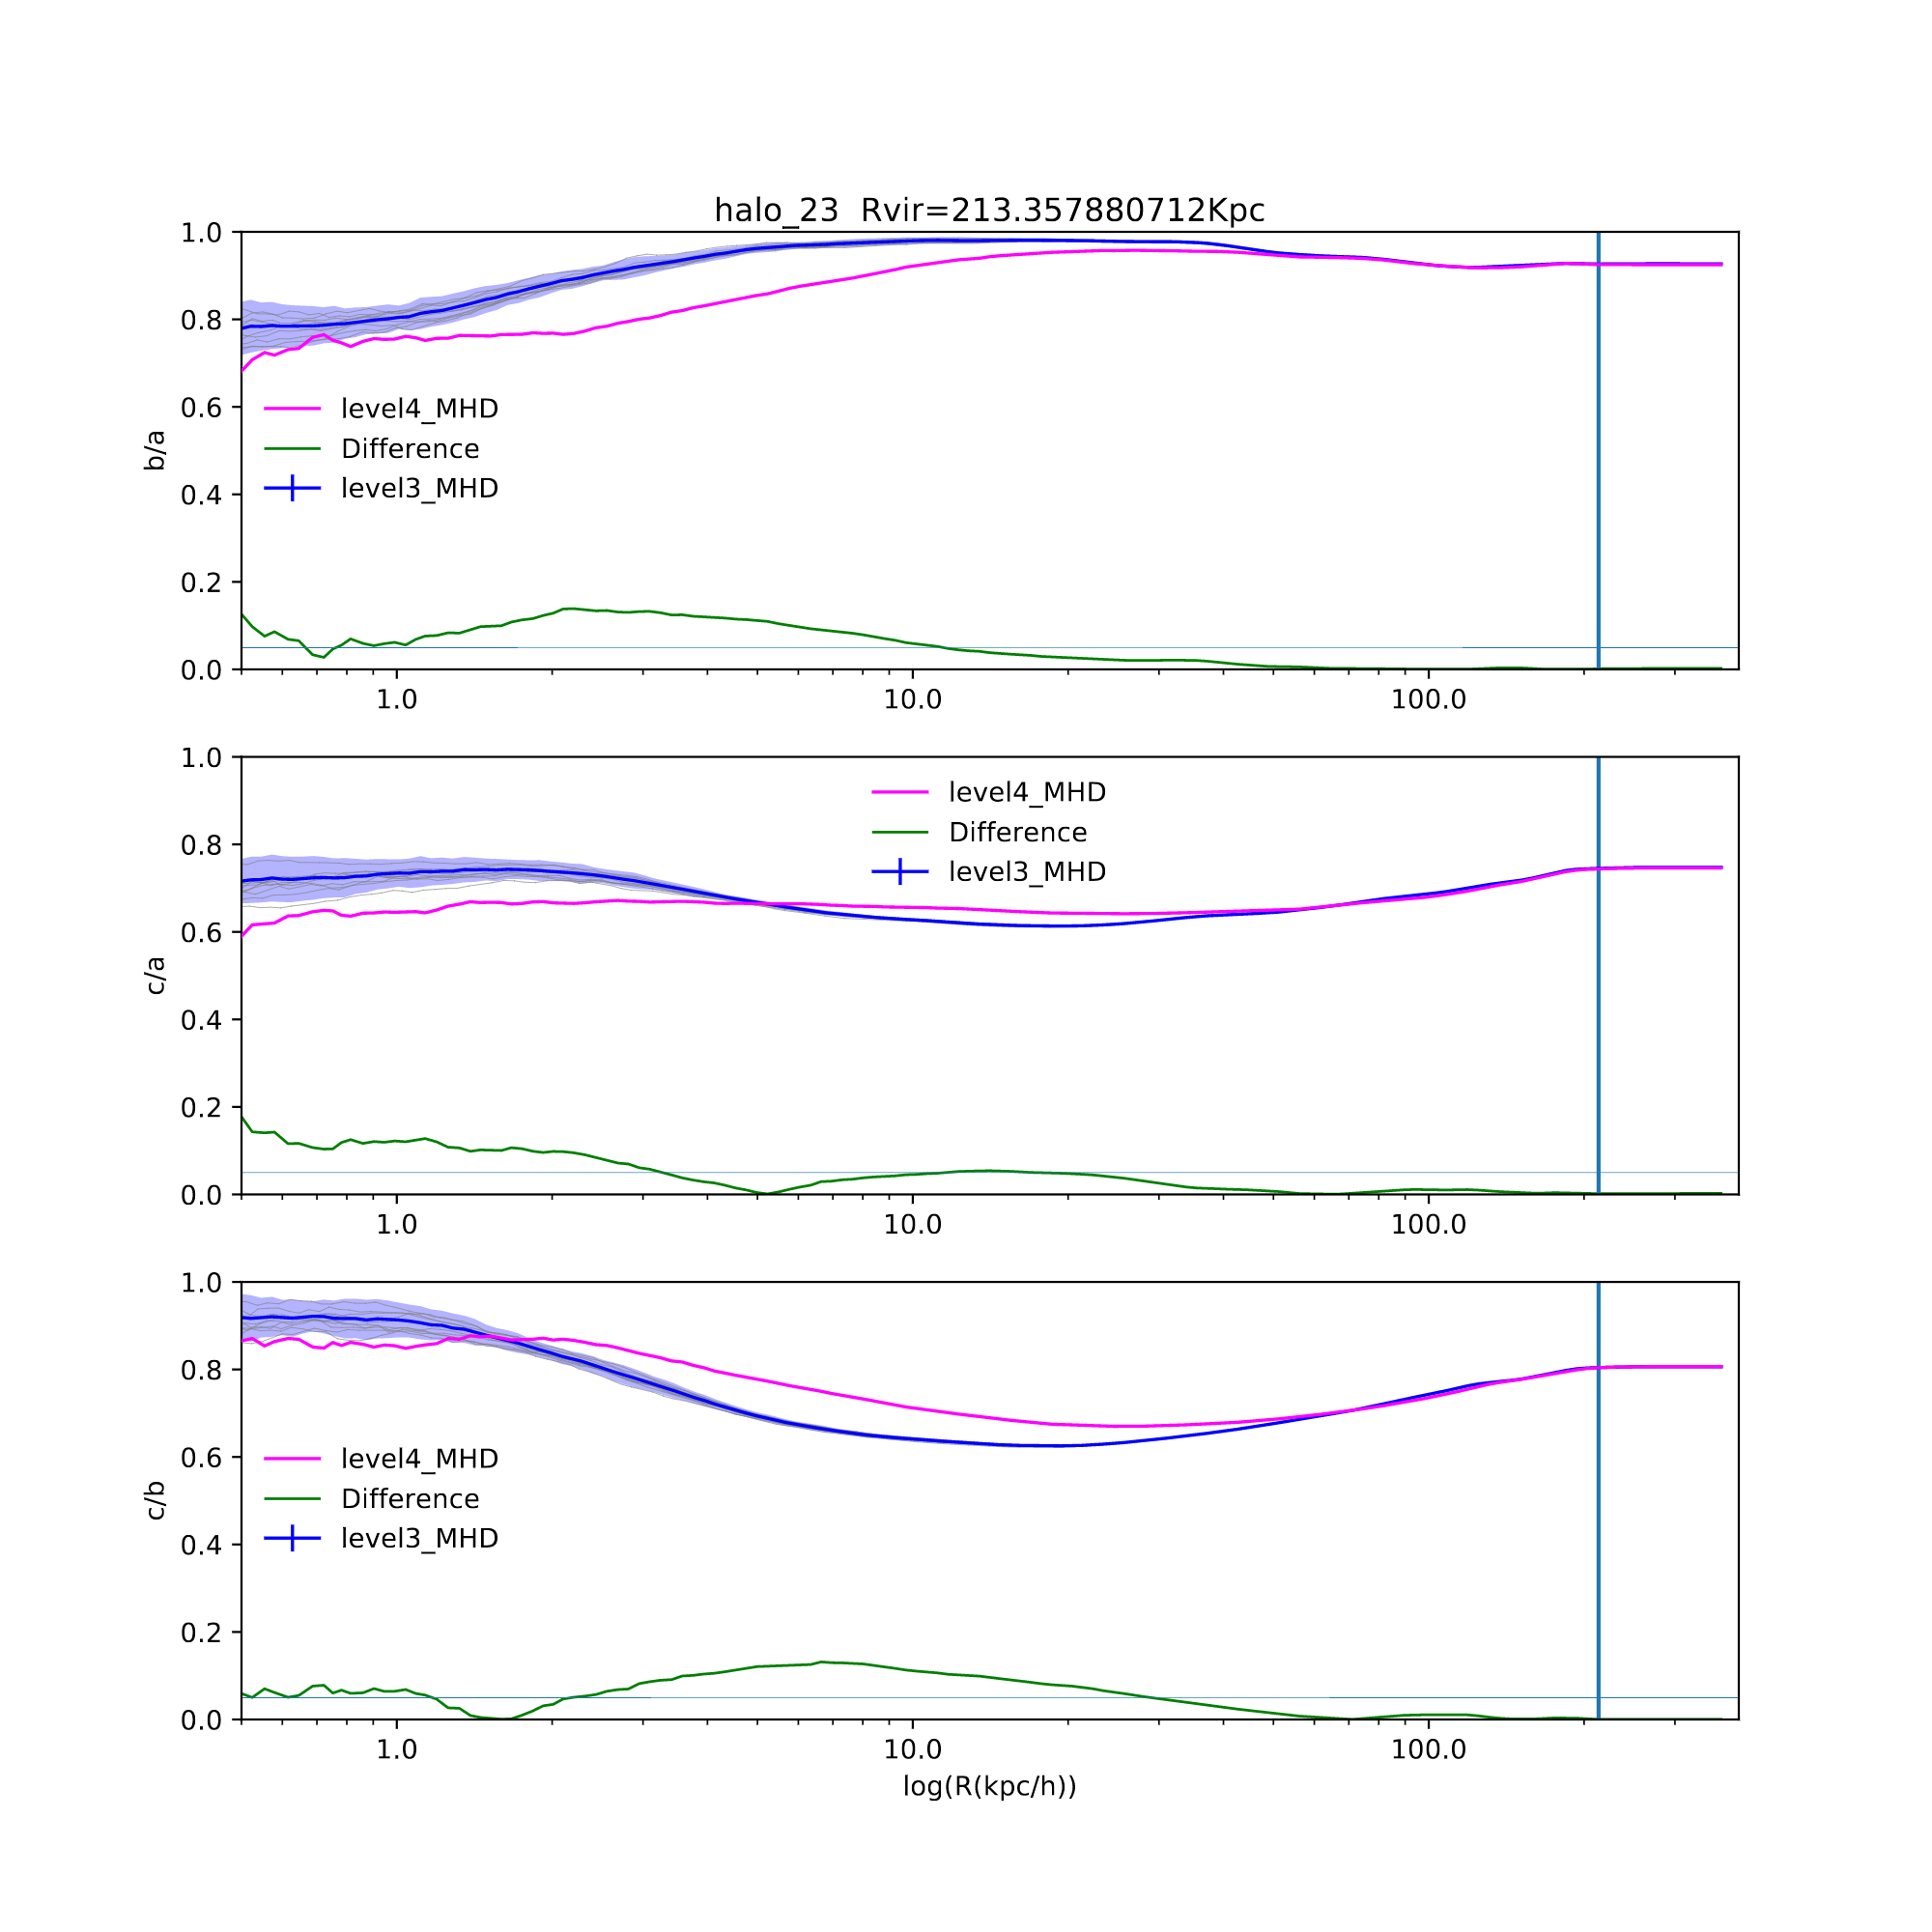
\includegraphics[width=0.4\textwidth]{./pics/Convergence23MHD.png}\label{fig:convergenceMHD}}
  \hfill
  \subfloat[DM]{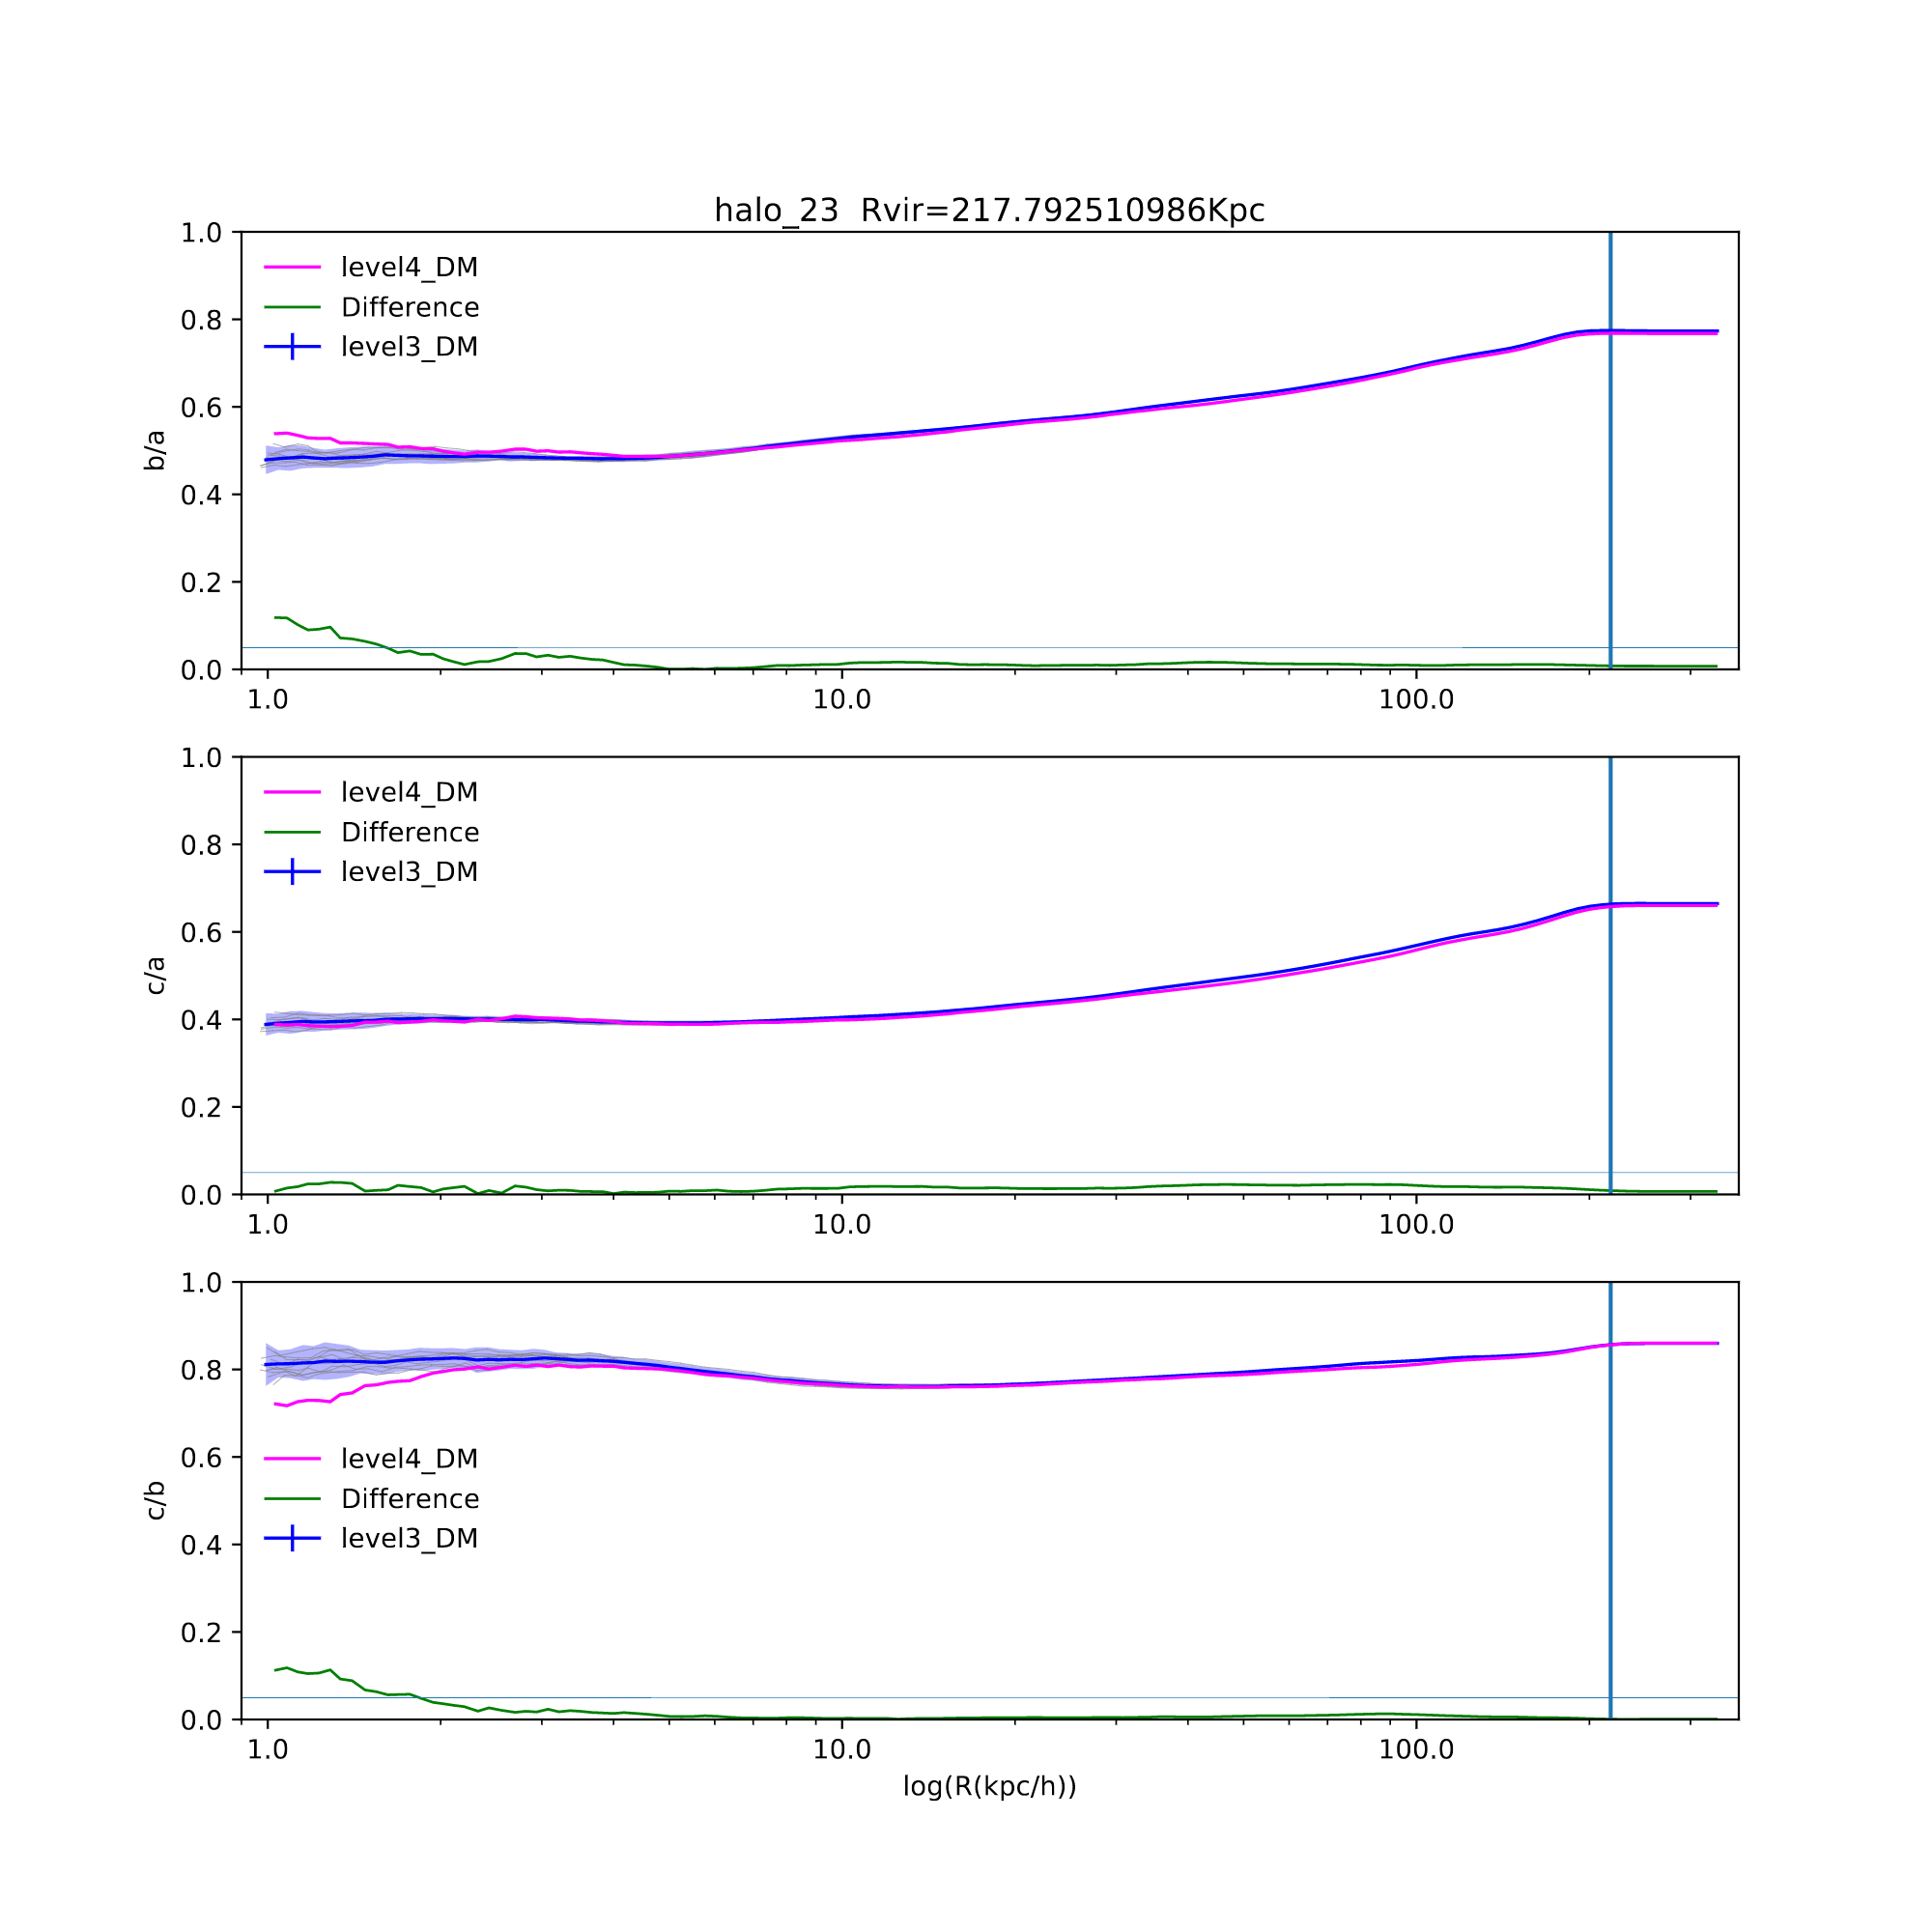
\includegraphics[width=0.4\textwidth]{./pics/Convergence23DM.png}\label{fig:convergenceDM}}
  \caption{Comparison of the effect of resolution on DM and MHD simualations. Here level4 curves (magenta) are compared to the mean and 2std (confirm) of the random-sampled curves from level3. For better comparison of the effect of resolution, the difference percent is plotted in green.  }
\end{figure}



State the main conclusions about this analysis of convergence. The effect of particle resolution does not sistematically affect the measurements. However, the error produced is specially apreciable at inner parts where for MHD it has a more global effect through scattering.\\

\section{Radial profiles}

Set the outline of the thesis



\section{The effect of gas on the halo shape}




\section{Historical shape}


 